\documentclass[12pt, a4paper]{article}

% ── Packages ──────────────────────────────────────────────────────────────────
\usepackage[utf8]{inputenc}
\usepackage[T1]{fontenc}
\usepackage[french]{babel}
\usepackage{geometry}
\geometry{margin=2.5cm}
\usepackage{graphicx}
\usepackage{booktabs}
\usepackage{amsmath}
\usepackage{hyperref}
\usepackage{caption}
\usepackage{float}
\usepackage{parskip}
\usepackage{setspace}
\onehalfspacing

\hypersetup{colorlinks=true, linkcolor=black, citecolor=black, urlcolor=black}

% ── Title ─────────────────────────────────────────────────────────────────────
\title{
    \vspace{-1cm}
    \Large \textbf{Commodity Trading Games} \\[0.4em]
    \large Marchés et Modèles de Matières Premières \\[0.4em]
    \normalsize ESILV -- Groupe G17 -- Café (KC=F) \\[0.4em]
    \normalsize Spring 2026
}
\author{Groupe G17}
\date{Mars 2026}

\begin{document}

\maketitle
\tableofcontents
\newpage

% ══════════════════════════════════════════════════════════════════════════════
\section{Analyse du secteur café et données}
% ══════════════════════════════════════════════════════════════════════════════

\subsection{Présentation du secteur}

Le café est l'une des matières premières agricoles les plus échangées au monde.
Le contrat de référence est le \textbf{Coffee C Futures (KC=F)}, coté sur
l'Intercontinental Exchange (ICE), qui représente 37~500 livres de café Arabica.
Son prix est influencé par les conditions climatiques au Brésil et en Colombie,
les taux de change, et la demande mondiale des grands groupes agroalimentaires.

L'univers d'actions retenu couvre l'ensemble de la chaîne de valeur du café :
torréfacteurs, distributeurs, groupes de restauration rapide et conglomérats
agroalimentaires exposés au prix du café.

\subsection{Sources de données}

Les données OHLCV journalières ont été téléchargées via l'API \texttt{yfinance}
pour la période du 1\textsuperscript{er} janvier 2020 au 28 février 2026,
soit plus de 5 ans de données. Le dataset contient 12 actifs :

\begin{itemize}
    \item \textbf{Anchor} : KC=F (Coffee C Futures)
    \item \textbf{Proxy ETF} : DBA (Invesco DB Agriculture Fund)
    \item \textbf{Actions} : SBUX, BROS, KDP, SJM, NSRGY, MDLZ, FARM, WEST
\end{itemize}

Deux tickers (JDEP, TAST) ont échoué au téléchargement car délistés.

\subsection{Nettoyage des données}

Les étapes de nettoyage appliquées sont les suivantes :
\begin{enumerate}
    \item Suppression des colonnes avec plus de 20\% de valeurs manquantes
    \item Remplissage des NaN restants par forward-fill
    \item Détection et neutralisation des outliers extrêmes ($|z\text{-score}| > 5$
          sur les rendements journaliers)
\end{enumerate}

La figure~\ref{fig:prices} montre l'évolution des prix normalisés (base 100)
de l'ensemble des actifs sur la période complète.

\begin{figure}[H]
    \centering
    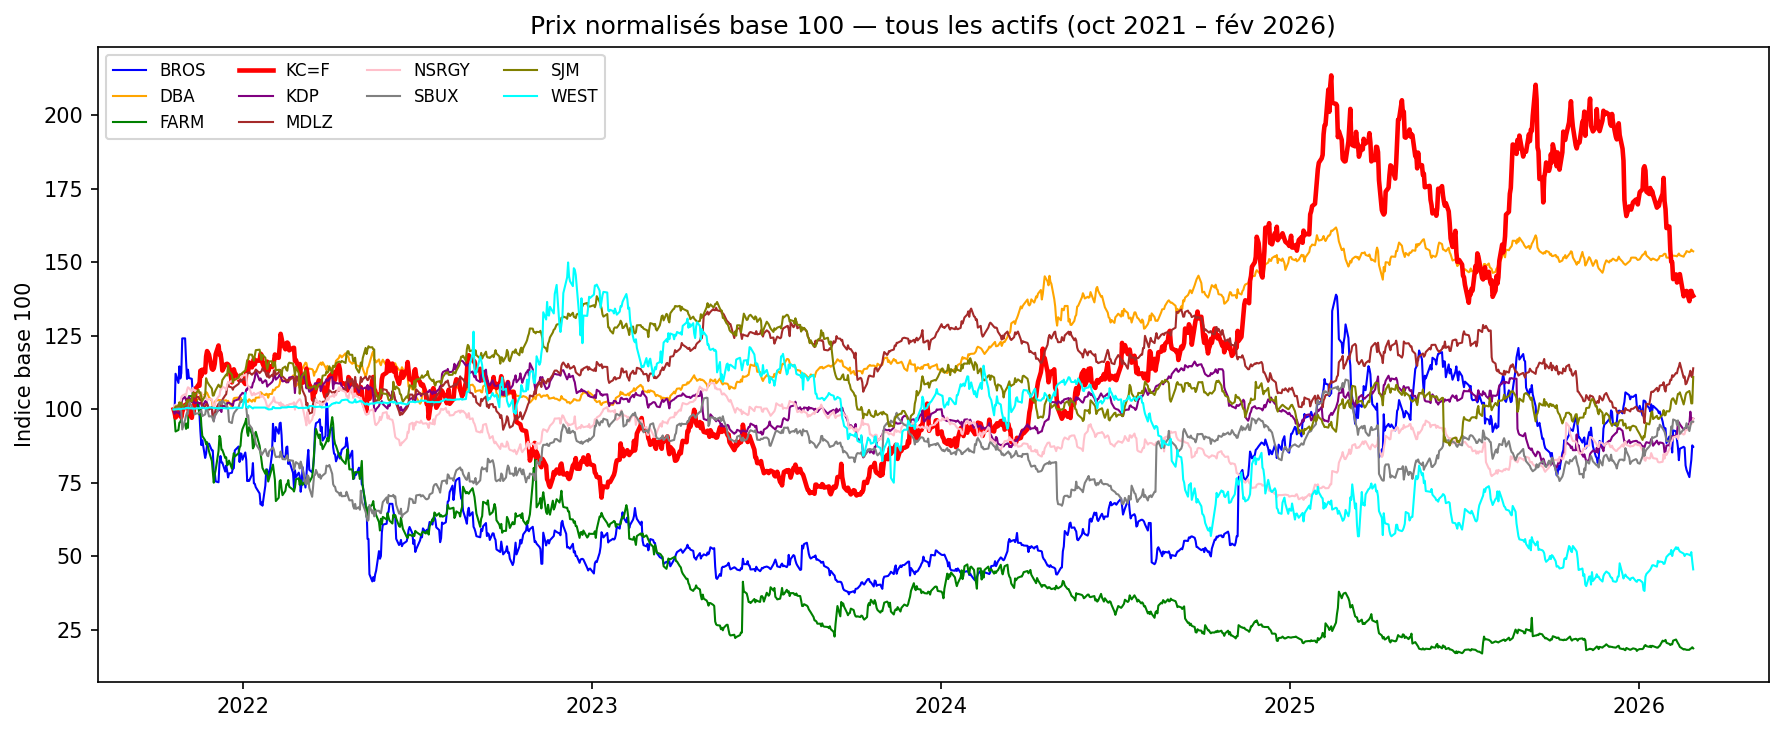
\includegraphics[width=\linewidth]{figures/fig_prices.png}
    \caption{Prix normalisés (base 100) -- Anchor, proxy et univers equity café}
    \label{fig:prices}
\end{figure}

\begin{figure}[H]
    \centering
    \includegraphics[width=0.85\linewidth]{figures/fig_correlation.png}
    \caption{Matrice de corrélation des rendements journaliers}
    \label{fig:corr}
\end{figure}

La matrice de corrélation (figure~\ref{fig:corr}) montre des corrélations
modérées entre KC=F et les actions du secteur, ce qui laisse de la place
pour de l'arbitrage statistique.

\newpage

% ══════════════════════════════════════════════════════════════════════════════
\section{Game \#1 -- Multivariate Pair Trading (Student A)}
% ══════════════════════════════════════════════════════════════════════════════

\subsection{Présentation de la stratégie}

La stratégie implémentée est un \textit{multivariate pair trading} market-neutral,
inspirée des travaux de \cite{yang2024}. L'objectif est de constituer un panier
d'actions dont l'exposition nette au marché café est nulle ($\sum \beta_i w_i = 0$),
et d'exploiter la mean-reversion du spread cointégré entre ce panier et l'anchor KC=F.

\subsection{Sélection du panier -- Tests de cointégration}

La période de \textbf{formation} couvre 2021--2022 et la période de
\textbf{trading} couvre 2023--2026.

Pour chaque action de l'univers, on applique le test d'Engle-Granger en deux étapes :
\begin{enumerate}
    \item Régression OLS des log-prix de l'action sur les log-prix de KC=F
    \item Test ADF sur les résidus (seuil $p < 0.10$)
\end{enumerate}

Le hedge ratio $\hat{\beta}$ issu de l'OLS mesure la sensibilité de chaque action
au futures café. Les 5 actions avec la $p$-value EG la plus faible sont retenues :
BROS, SJM, SBUX, MDLZ, KDP.

\subsection{Optimisation Gurobi -- Neutralité marché}

Les poids optimaux $w^*$ sont obtenus en résolvant le problème quadratique suivant :

\begin{equation}
    \min_{w} \; w^\top \Sigma w
    \quad \text{s.t.} \quad
    \sum_{i} \beta_i w_i = 0, \quad \sum_{i} w_i = 1, \quad w_i \in [-1, 1]
\end{equation}

où $\Sigma$ est la matrice de covariance des rendements log sur la période de
formation, et $\beta_i$ est le hedge ratio de l'action $i$ estimé par OLS.

La contrainte $\sum \beta_i w_i = 0$ garantit la \textbf{neutralité marché} :
le portefeuille n'a aucune exposition nette aux futures café.
Le solveur utilisé est \texttt{gurobipy} (licence académique Gurobi 13.0.1).

\begin{figure}[H]
    \centering
    \includegraphics[width=0.75\linewidth]{figures/fig_weights.png}
    \caption{Poids optimaux du basket market-neutral -- bleu = long, rouge = short}
    \label{fig:weights}
\end{figure}

Le net beta obtenu est $\sum \beta_i w_i = 0.000000$, confirmant la contrainte
de neutralité marché.

\subsection{Backtest -- Mean reversion sur Z-score}

Le spread du panier est défini comme :

\begin{equation}
    S_t = \sum_{i} w_i \ln P_{i,t}
\end{equation}

Le Z-score rolling (fenêtre de 60 jours) est calculé comme :

\begin{equation}
    Z_t = \frac{S_t - \mu_{t,60}}{\sigma_{t,60}}
\end{equation}

Les règles de trading sont les suivantes :
\begin{itemize}
    \item \textbf{Entrée long} : $Z_t < -2$ (spread sous-évalué)
    \item \textbf{Entrée short} : $Z_t > +2$ (spread sur-évalué)
    \item \textbf{Sortie} : $Z_t$ revient à 0
    \item \textbf{Coûts de transaction} : 10 bps par leg
\end{itemize}

\subsection{Résultats}

\begin{figure}[H]
    \centering
    \includegraphics[width=\linewidth]{figures/fig_results.png}
    \caption{Courbe de valeur, drawdown et signaux Z-score (2023--2026)}
    \label{fig:results}
\end{figure}

\begin{figure}[H]
    \centering
    \includegraphics[width=\linewidth]{figures/fig_monthly_pnl.png}
    \caption{PnL mensuel de la stratégie OTT basket}
    \label{fig:pnl}
\end{figure}

\begin{table}[H]
\centering
\caption{Métriques de performance -- Période de trading 2023--2026}
\begin{tabular}{lcc}
\toprule
\textbf{Métrique} & \textbf{OTT Basket (Gurobi)} & \textbf{Benchmark EW} \\
\midrule
Rendement annualisé (\%)  & $-2.57$  & $+3.03$  \\
Volatilité annualisée (\%) & $7.14$  & $18.20$  \\
Sharpe Ratio               & $-0.889$ & $0.035$  \\
Max Drawdown (\%)          & $-10.91$ & $-21.36$ \\
Calmar Ratio               & $-0.235$ & $0.141$  \\
Nombre de trades           & $11$     & $1$      \\
Win Rate (\%)              & $54.55$  & --       \\
\bottomrule
\end{tabular}
\label{tab:perf}
\end{table}

\subsection{Analyse de sensibilité}

\begin{figure}[H]
    \centering
    \includegraphics[width=\linewidth]{figures/fig_sensitivity.png}
    \caption{Sensibilité des métriques au seuil Z d'entrée}
    \label{fig:sensitivity}
\end{figure}

L'analyse de sensibilité (figure~\ref{fig:sensitivity}) montre que le seuil
$Z = 2.0$ offre un bon compromis entre nombre de trades et qualité des signaux.

\subsection{Discussion}

La stratégie présente une \textbf{volatilité significativement plus faible}
que le benchmark (7.14\% vs 18.20\%) et un \textbf{drawdown maximal deux fois
moindre} ($-10.91\%$ vs $-21.36\%$), confirmant l'efficacité de la
contrainte de neutralité marché.

Le rendement négatif sur 2023--2026 s'explique par la faible volatilité du
spread cointégré sur cette période, limitant les opportunités d'arbitrage.
Le marché du café a connu une tendance haussière prononcée, défavorable
aux stratégies mean-reversion.

La principale limite est l'estimation statique des hedge ratios sur la
période de formation, qui peut souffrir d'instabilité structurelle hors échantillon.

% ══════════════════════════════════════════════════════════════════════════════
\begin{thebibliography}{9}

\bibitem{yang2024}
Yang, H., \& Malik, A. (2024).
\textit{Optimal market-neutral multivariate pair trading on the cryptocurrency platform}.
International Journal of Financial Studies, 12(3), 77.

\bibitem{engle1987}
Engle, R. F., \& Granger, C. W. J. (1987).
\textit{Co-Integration and Error Correction}.
Econometrica, 55(2), 251--276.

\bibitem{markowitz1952}
Markowitz, H. (1952).
\textit{Portfolio Selection}.
The Journal of Finance, 7(1), 77--91.

\end{thebibliography}

\end{document}
